\documentclass{pracamgr}

\usepackage{polski}
\usepackage[utf8]{inputenc}
\usepackage{graphicx}

\usepackage{subfig} % Subfigures

\author{Maciej Pazurkiewicz}
\nralbumu{248267}

\title{Modelowanie sygnalizacji świetlnej}

\tytulang{Modelling of a traffic lights system}
\kierunek{Informatyka}

\opiekun{dra hab. Sławomira Lasoty\\
  Instytut Informatyki
  }
% miesiąc i~rok:
\date{Wrzesień 2011}

%Podać dziedzinę wg klasyfikacji Socrates-Erasmus:
\dziedzina{ 
11.3 Informatyka\\ 
}

%Klasyfikacja tematyczna wedlug AMS (matematyka) lub ACM (informatyka)
\klasyfikacja{D. Software\\
  D.2. Software engineering\\
  D.2.4. Software/Program verification}

% Słowa kluczowe:
\keywords{}

% Moje makra
\newtheorem{defi}{Definicja}[section]
\newcommand{\ang}[1]{(ang.~\emph{#1})}

\begin{document}
\maketitle

\begin{abstract}
streszczenie
\end{abstract}

\tableofcontents

\chapter*{Wprowadzenie}
\addcontentsline{toc}{chapter}{Wprowadzenie}

\chapter{Sygnalizacja świetlna}
\label{c:sygnalizacja}

Niniejszy rozdział zawiera opis systemów sygnalizacji świetlnej, które
będą modelowane blabla. Jest on oparty na raportach przygotowanych na
zlecenie amerykańskiej agencji \emph{Federal Highway Administration}
\cite{timing} \cite{handbook}.

\section{Wprowadzenie}
\label{s:sygn-wprowadzenie}

Sygnalizacją świetlną nazywamy zestaw urządzeń przekazujących
komunikaty, służące do segregacji czasowej kolidujących potoków
ruchu. Stosuje się ją najpowszechniej na skrzyżowaniach i przejściach
dla pieszych, lecz wykorzystywana jest także w miejscach takich jak
przejazdy kolejowe, drogi o ruchu wahadłowym lub drogi o pasach o
zmiennym kierunku ruchu.

Poprawnie zaprojektowana sygnalizacja świetlna powinna zmniejszać
prawdopodobieństwo wypadków i kolizji oraz zapewniać odpowiedni poziom
dostępności dla pieszych i pojazdów nadjeżdżających z kierunków
podporządkowanych, jednocześnie zachowując jak największą wydajność
skrzyżowania (tj. maksymalizować jego przepustowość i minimalizować
czas oczekiwania na sygnał zielony).  Zapewnienie równowagi pomiędzy
bezpieczeństwem a wydajnością należy do kluczowych elementów projektu
sygnalizacji.

\subsection{Elementy systemu sygnalizacji świetlnej}
\label{ss:elementy}
Najprostszy system sygnalizacji składa się z sygnalizatora oraz
kontrolera, czyli układu logicznego decydującego o wyświetlanym
sygnale. Współczesne systemy są często o wiele bardziej skomplikowane
i mogą zawierać komponenty takie jak:
\begin{description}
  \item[czujniki] -- urządzenia, które zbierają informację o aktualnym
  zapotrzebowaniu na prawo przejazdu bądź przejścia różnych
  uczestników ruchu, np. pętle indukcyjne w jezdni dla pojazdów bądź
  przyciski dla pieszych;
  \item[kontroler lokalny] -- urządzenie zarządzające pracą grupy
  ściśle powiązanych sygnalizatorów, np. sterujących ruchem na jednym
  skrzyżowaniu;
  \item[kontroler główny] -- urządzenie zarządzające pracą grupy
  kontrolerów lokalnych; może być odpowiedzialny np. za synchronizację
  sygnalizacji na ciągu skrzyżowań.
\end{description}

\subsection{Tryby pracy}
\label{ss:tryby}
Sygnalizacja świetlna na skrzyżowaniach pracuje przeważnie w trybie
stałoczasowym, wzbudzanym lub kombinacji obydwu.

\paragraph{Sygnalizacja stałoczasowa}
W trybie stałoczasowym każdy z sygnałów dla każdego potoku ma z góry
określoną długość.

\paragraph{Sygnalizacja wzbudzana}
W trybie wzbudzanym kontroler korzysta z informacji dostarczanych
przez czujniki, dzięki czemu może dostosować parametry pracy
sygnalizacji do aktualnych warunków ruchu. W zależności od tego czy
czujniki są zainstalowane dla wszystkich potoków czy tylko dla
niektórych mówimy o sygnalizacji \emph{w pełni wzbudzanej}
\ang{fully-actuated } lub \emph{częściowo wzbudzanej}
\ang{semi-actuated}.

W systemach w pełni wzbudzanych sygnalizacja dla każdego z potoków
jest uzależniona od danych dostarczonych przez czujnik. W
szczególności oznacza to, że w danym cyklu sygnał zielony otrzymują
tylko te fazy, na które jest zapotrzebowanie. Co więcej długość
sygnału zielonego może być uzależniona od liczby oczekujących pojazdów.

W systemach częściowo wzbudzanych detekcja ruchu dotyczy tylko
niektórych potoków ruchu, np. pieszych bądź pojazdów nadjeżdżających z
drogi podrzędnej. Prawo przejazdu jest domyślnie przyznawane
kierunkowi głównemu; pozostałe zaś mogą je otrzymać w wyniku
zapotrzebowania zgłoszonego przez czujnik.

\section{Szczegółowy opis funkcjonowania wybranych systemów}
\label{s:szczegoly}

\subsection{Podstawowe pojęcia}
 \label{ss:pojecia}

\begin{description}
  \item[interwał] -- odcinek czasu, w którym wskazanie danego
  sygnalizatora nie zmienia się;
  \item[potok ruchu] -- pojazdy bądź piesi, których ruch kontrolowany
  jest przez jeden sygnalizator;
  \item[faza] -- grupa potoków ruchu, które mogą jednocześnie
  korzystać ze skrzyżowania; może składać się z:
  \begin{itemize}
    \item jednego lub więcej potoku pojazdów,
    \item jednego lub więcej potoku pieszych,
    \item kombinacji pewnej liczby potoków samochodowych i pieszych;
  \end{itemize}
  \begin{figure}[h]
    \centering
    \subfloat[Faza wyłącznie dla pojazdów]{
      
\includegraphics[width=0.27\textwidth]{img/signals-phase-example-1}
    }
    \hfill
    \subfloat[Faza dla pojazdów oraz pieszych]{
      \includegraphics[width=0.27\textwidth]{img/signals-phase-example-2}
    }
    \hfill
    \subfloat[Faza wyłącznie dla pieszych \ang{pedestrian scramble, X~crossing}]{
      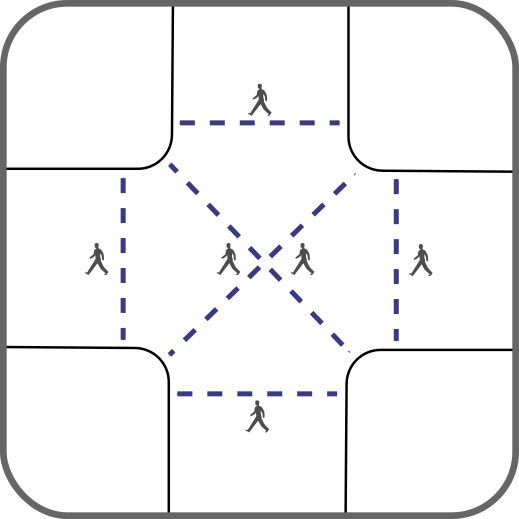
\includegraphics[width=0.27\textwidth]{img/signals-phase-example-3}
    }
    \caption{Przykładowe fazy}
  \end{figure}
  \item[cykl] -- ustalony ciąg faz
  \begin{figure}[h]
    \centering
    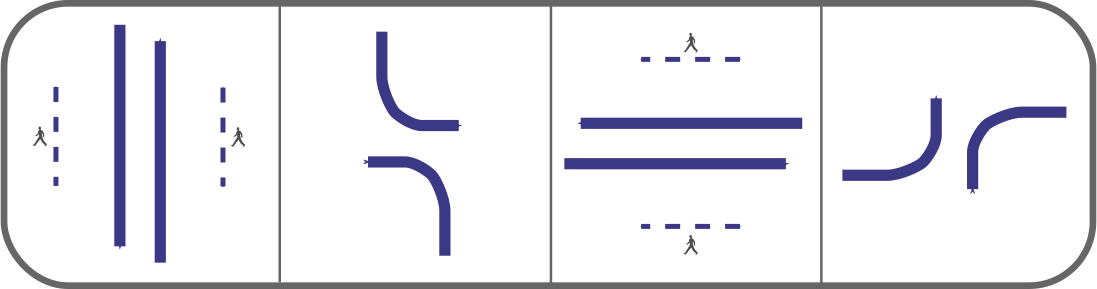
\includegraphics[width=0.7\textwidth]{img/signals-cycle-example}
    \caption{Przykładowy cykl}
  \end{figure}
\end{description}



\subsection{Sygnalizacja stałoczasowa}
\subsection{Sygnalizacja wzbudzana}

\subsubsection{Detekcja ruchu}
\label{ss:detekcja}

\subsubsection{Opis i parametry systemu}
\label{sec:opis-parametry}
Wykrycie pojazdu przez czujnik powoduje zgłoszenie żądania i włączenie
sygnału zielonego. Sygnał ten jest przedłużany, o ile wykrywane są
następne pojazdy. Jego koniec następuje, jeśli pomiędzy
nadjeżdżającymi pojazdami jest luka o dostatecznie dużej długości
\ang{\mbox{gap-out}} bądź został osiągnięty maksymalny czas sygnału
zielonego dla danego kierunku \ang{\mbox{max-out}}. Druga opcja brana
jest pod uwagę wyłącznie wtedy, gdy wcześniej otrzymano zgłoszenie dla
kolidującego kierunku ruchu.

W celu formalizacji powyższego opisu wprowadzamy następujące definicje:%
\begin{description}
  \item[minimalny zielony] \ang{minimal green} -- najkrótszy
  \item[maksymalny zielony] \ang{maximal green} -- najdłuższy czas,
  przez który dany ruch może otrzymywać zielony sygnał w obecności
  zgłoszenia przeciwnego
  \item[wydłużenie] \ang{passage time} -- czas, o który wydłużany jest
  sygnał zielony po wzbudzeniu czujnika; brak wzbudzenia czujnika
  przez ten czas powoduje wyłączenie sygnału zielonego
\end{description}

\subsubsection{Schemat funkcjonowania podstawowego systemu sygnalizacji wzbudzanej dla pojazdów}
\label{ss:wzbudzana-schemat}

Podstawowy system pełni wzbudzanej sygnalizacji dla pojazdów oparty
jest na następujących założeniach:
\begin{enumerate}
  \item sygnał zielony dla danego ruchu włączany jest wyłącznie w
  wyniku realizacji żądania
  \item czujniki umieszczone są na linii zatrzymania się pojazdów i
  pracują w trybie pulsacyjnym z pamięcią; 
  \item wartości parametrów minimalny i maksymalny zielony oraz
  wydłużenie są stałe
  \item długości interwałów czerwono-żółtego, żółtego i czerwonego
  odstępu są stałe
\end{enumerate}
W celu realizacji powyższych założeń dzielimy interwał zielony na dwie
części \emph{początkową} oraz \emph{rozszerzalną}

\begin{thebibliography}{99}
\addcontentsline{toc}{chapter}{Bibliografia}

% http://ops.fhwa.dot.gov/publications/fhwahop06006/form_dot_1700.htm
\bibitem[FHWA06]{handbook} Robert L. Gordon, Warren Tighe,
\textit{Traffic Control Systems Handbook}, Federal Highway
Administration, 2006.

% http://ops.fhwa.dot.gov/publications/fhwahop08024/doc_page.htm
\bibitem[FHWA08]{timing} Peter Koonce i in., \textit{Traffic Signal
  Timing Manual}, Federal Highway Administration, 2008.

\end{thebibliography}

\end{document}

%%% Local Variables:
%%% mode: latex
%%% TeX-master: t
%%% coding: utf-8
%%% eval: (auto-fill-mode 1)
%%% End:
